\documentclass[12pt]{article}

\usepackage[top=2.2cm,bottom=2.5cm,left=2.5cm,right=2.5cm]{geometry}
\usepackage{amsmath,amssymb,amsfonts,amsthm}
\usepackage{graphicx}
\usepackage{float}
\usepackage{fancyhdr}
\usepackage{tikz}
\usetikzlibrary{trees,arrows.meta,positioning}
\usepackage{algorithm}
\usepackage{algpseudocode}
\usepackage{tabularx,array,xcolor,colortbl}
\usepackage{enumitem}
\usepackage{hyperref}
\hypersetup{
    colorlinks=true,
    linkcolor=blue,
    urlcolor=blue,
}
\usepackage[nameinlink]{cleveref}

\newcolumntype{C}[1]{>{\centering\arraybackslash}p{#1}}

\usepackage{xepersian}
\settextfont[
  Path = fonts/,
  Extension = .ttf,
  UprightFont = *-Regular,
  BoldFont = *-Bold
]{Vazirmatn}
\setlatintextfont{Times New Roman}

\setlength{\headheight}{23pt}
\renewcommand{\baselinestretch}{1.3}
\setlength{\parindent}{0pt}
\setlength{\parskip}{5pt}

\pagestyle{fancy}
\fancyhf{}
\renewcommand{\headrulewidth}{0.8pt}
\fancyhead[R]{\scriptsize درس نرم افزار ریاضی}
\fancyhead[C]{\scriptsize پروژه سوم}
\fancyhead[L]{
\includegraphics[width=0.65cm]{fa-logo.png}} 
\fancyfoot[C]{\thepage}

\setlength{\headheight}{24pt}
\addtolength{\topmargin}{-1pt}

\begin{document}

\begin{titlepage}
\centering
\vspace*{0.5cm}

\includegraphics[width=4cm]{fa-logo.png}\\[0.7cm]
{\Large\textbf{دانشگاه صنعتی امیرکبیر}}\\[1mm]
{\normalsize (پلی‌تکنیک تهران)}\\[3mm]
{\large دانشکده ریاضی و علوم کامپیوتر}\\[3cm]

{\huge\textbf{پروژه سوم}}\\[0.8cm]
{\large درس نرم افزار ریاضی}\\[2.5cm]

{\normalsize
استاد درس: دکتر امین حسینقلی‌زاده\\[0.6em]
تیر ۱۴۰۵
}\\[2.5cm]

{\normalsize
نام و نام خانوادگی: پارسا نصیری\\[0.5em]
کد دانشجویی: ۴۰۲۱۲۰۴۷
}
\end{titlepage}

\newpage
\setcounter{page}{2}

\tableofcontents

\newpage

\section{مقدمه}

در این پروژه سه مبحث مهم از درس نرم‌افزار ریاضی مورد بررسی قرار گرفته است. در بخش اول، روش‌های درونیابی لاگرانژ و اسپلاین مکعبی برای تقریب مجموعه‌ای از داده‌های گسسته پیاده‌سازی و با یکدیگر مقایسه شده‌اند. در بخش دوم، داده‌های موجود در یک فایل اکسل با استفاده از کتابخانه‌های پایتون خوانده شده و نمودارهای مختلفی برای تحلیل زمان اجرای الگوریتم‌ها ترسیم شده است. همچنین میانگین زمان اجرای یکی از الگوریتم‌ها محاسبه شده است.

در بخش سوم، انتگرال معین تابع
\[
f(x)=e^{x^2}
\]
بر روی بازه $[0,1]$ با استفاده از روش‌های عددی مختلف شامل روش ذوزنقه‌ای، روش سیمپسون و انتگرال‌گیری گاوسی محاسبه شده و نتایج حاصل با یکدیگر مقایسه شده‌اند.

تمامی پیاده‌سازی‌ها با استفاده از زبان برنامه‌نویسی Python و کتابخانه‌های علمی آن انجام شده است. همچنین تمامی نمودارها و خروجی‌های مورد نیاز تولید و در این گزارش به همراه تحلیل نتایج ارائه شده‌اند.

\section{سؤال اول}

\subsection{صورت مسئله}

در این بخش، مجموعه نقاط

\[
(1,1),\;
(2,3),\;
(3,5),\;
(4,8),\;
(5,5),\;
(6,2)
\]

داده شده‌اند. هدف، درونیابی این داده‌ها با استفاده از دو روش لاگرانژ و اسپلاین مکعبی و سپس مقایسه نتایج حاصل از این دو روش است. علاوه بر رسم نمودارها، ضابطه چندجمله‌ای لاگرانژ و چندجمله‌ای‌های قطعه‌ای اسپلاین نیز محاسبه شده‌اند.

\subsection{پیاده‌سازی}

ابتدا داده‌های مسئله به صورت آرایه‌های NumPy تعریف شدند. سپس با استفاده از کتابخانه \lr{SymPy} چندجمله‌ای درونیاب لاگرانژ محاسبه گردید. برای درونیابی اسپلاین نیز از کلاس \lr{CubicSpline} موجود در کتابخانه \lr{SciPy} استفاده شد.

پس از محاسبه توابع درونیاب، هر دو تابع روی یک بازه یکنواخت نمونه‌برداری شده و نمودارهای مربوطه رسم شدند. در انتها نیز ضرایب هر قطعه از اسپلاین مکعبی استخراج و نمایش داده شدند تا فرم دقیق توابع قطعه‌ای مشخص شود.

\subsection{درونیابی لاگرانژ}

شکل~\ref{fig:lagrange} نمودار حاصل از درونیابی لاگرانژ را نشان می‌دهد.

\begin{figure}[H]
\centering
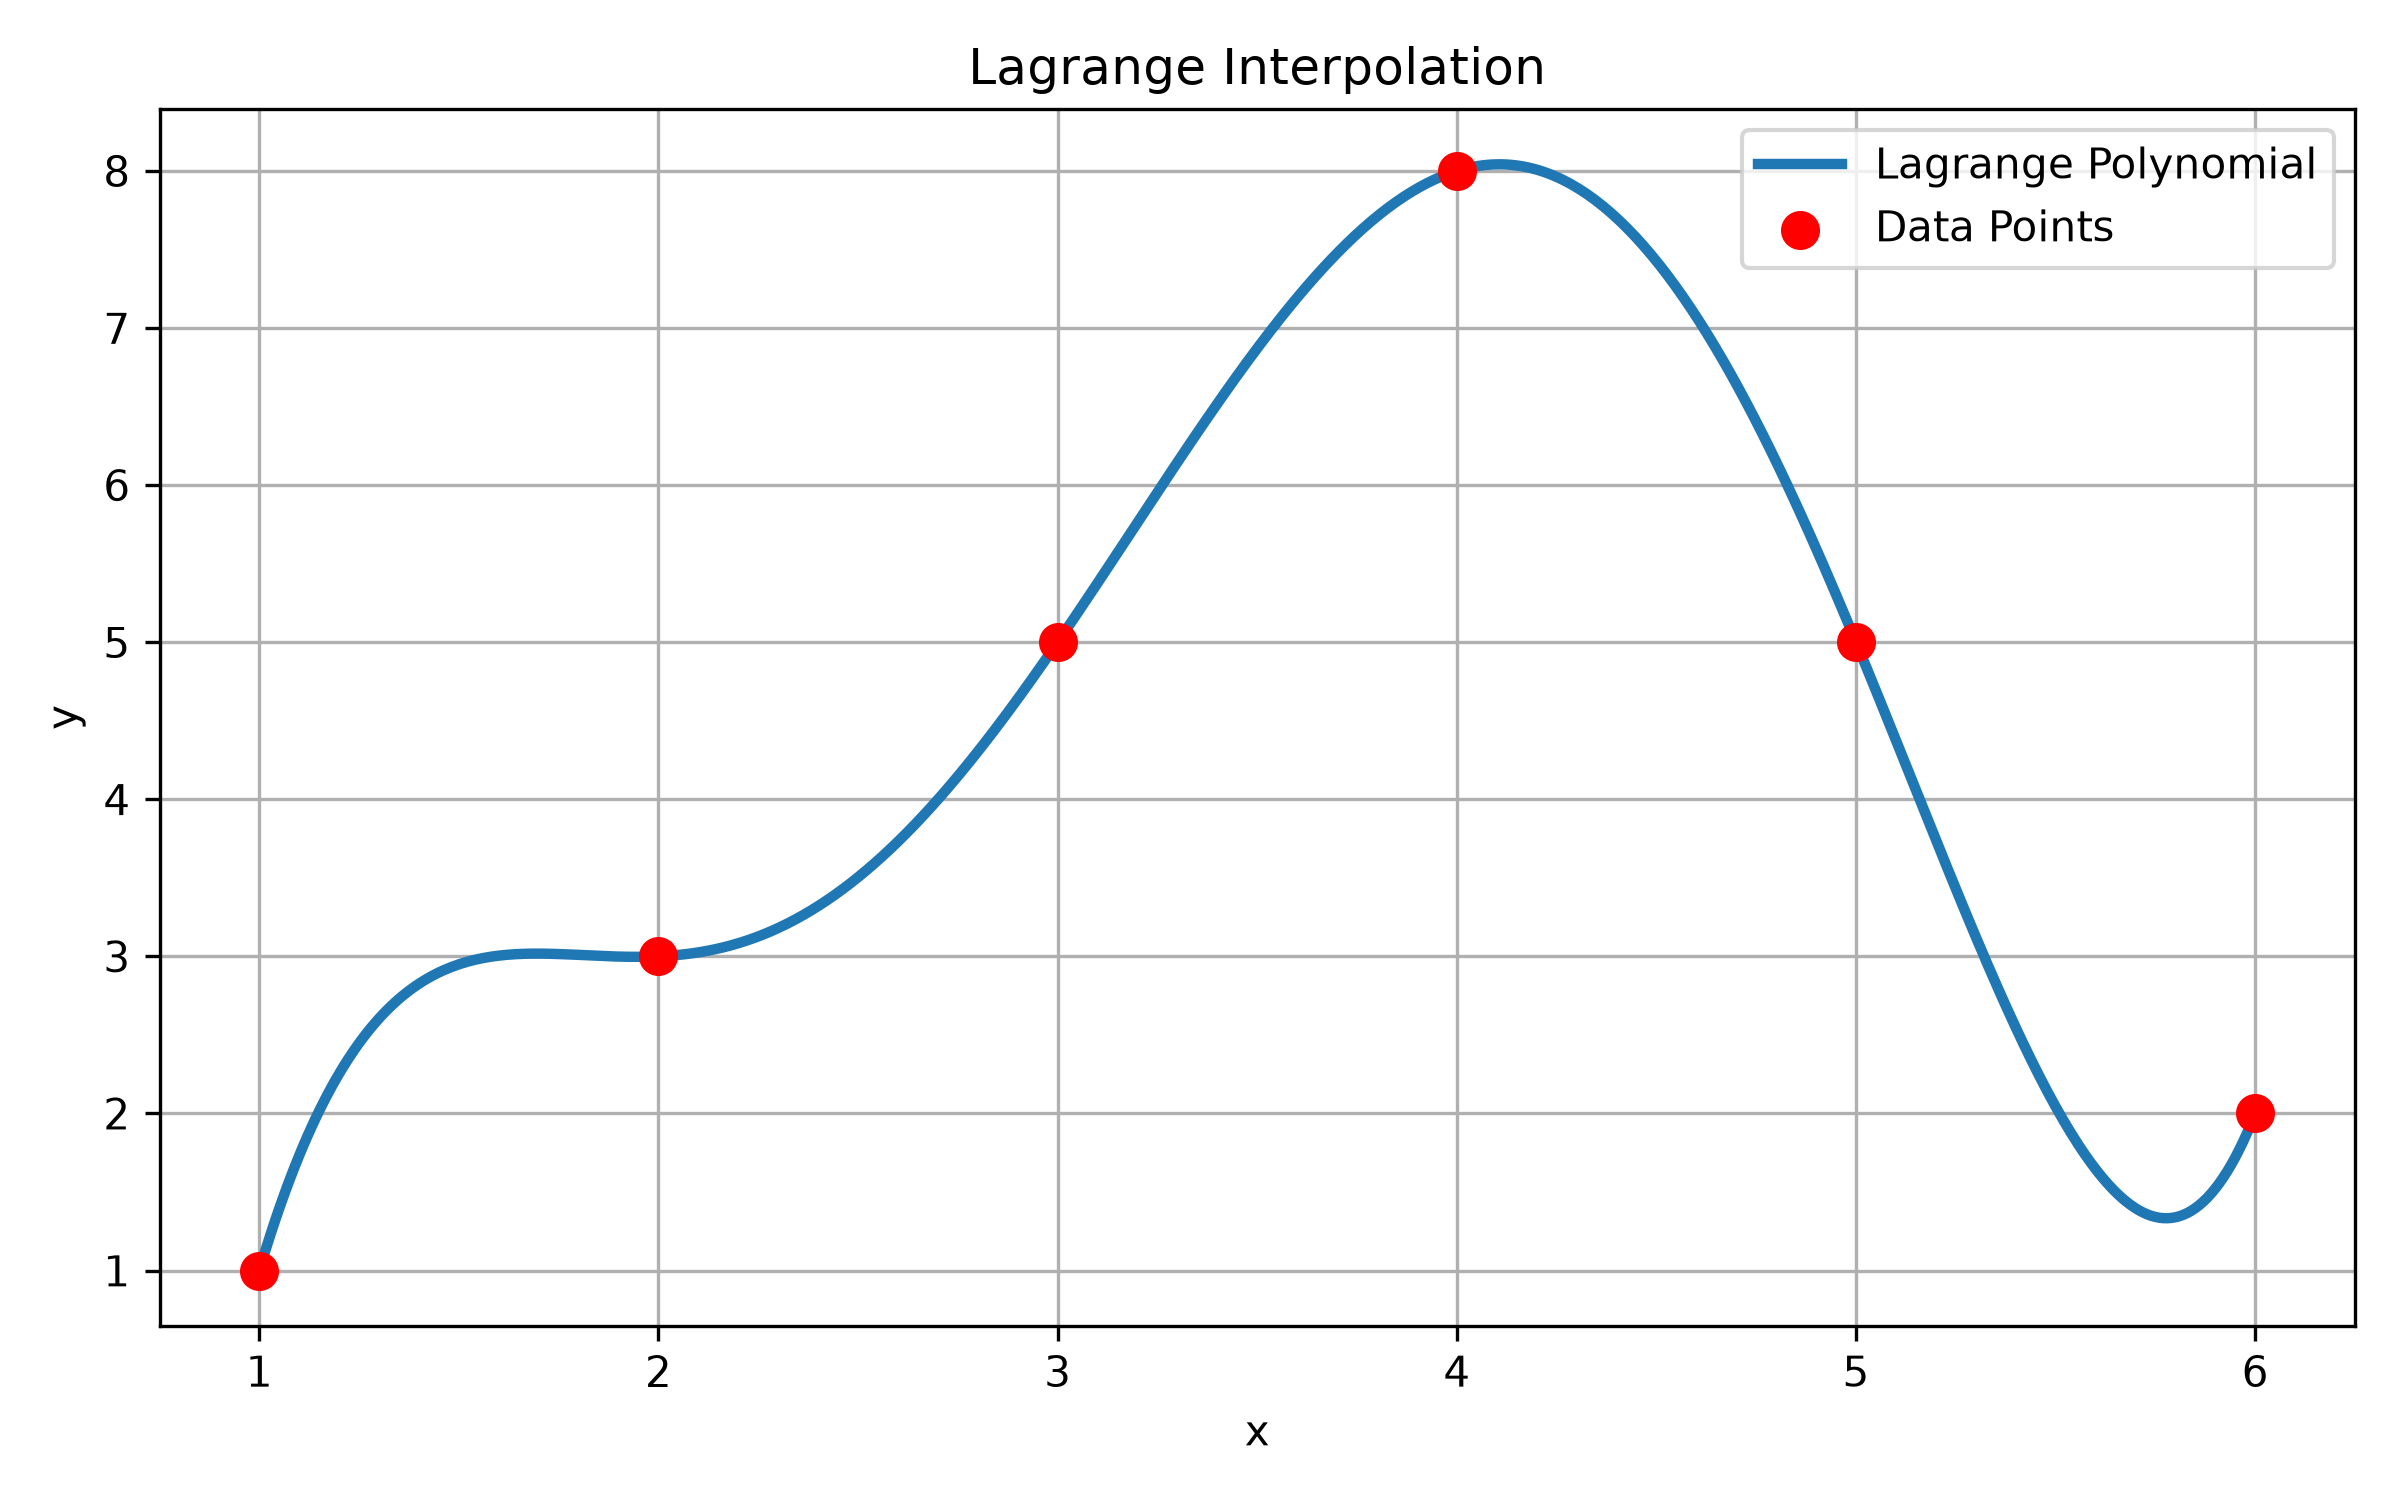
\includegraphics[width=0.82\textwidth]{figures/lagrange.png}
\caption{Lagrange interpolation}
\label{fig:lagrange}
\end{figure}

در این روش، یک چندجمله‌ای درجه پنج از تمامی نقاط عبور می‌کند. بنابراین مقدار تابع در تمام نقاط داده‌شده دقیقاً برابر مقادیر اولیه خواهد بود. اگرچه این روش در مجموعه داده‌های کوچک عملکرد مناسبی دارد، اما با افزایش تعداد نقاط، درجه چندجمله‌ای نیز افزایش یافته و احتمال ایجاد نوسانات ناخواسته در بین نقاط بیشتر می‌شود.

\subsection{درونیابی اسپلاین مکعبی}

شکل~\ref{fig:spline} نتیجه درونیابی اسپلاین مکعبی را نمایش می‌دهد.

\begin{figure}[H]
\centering
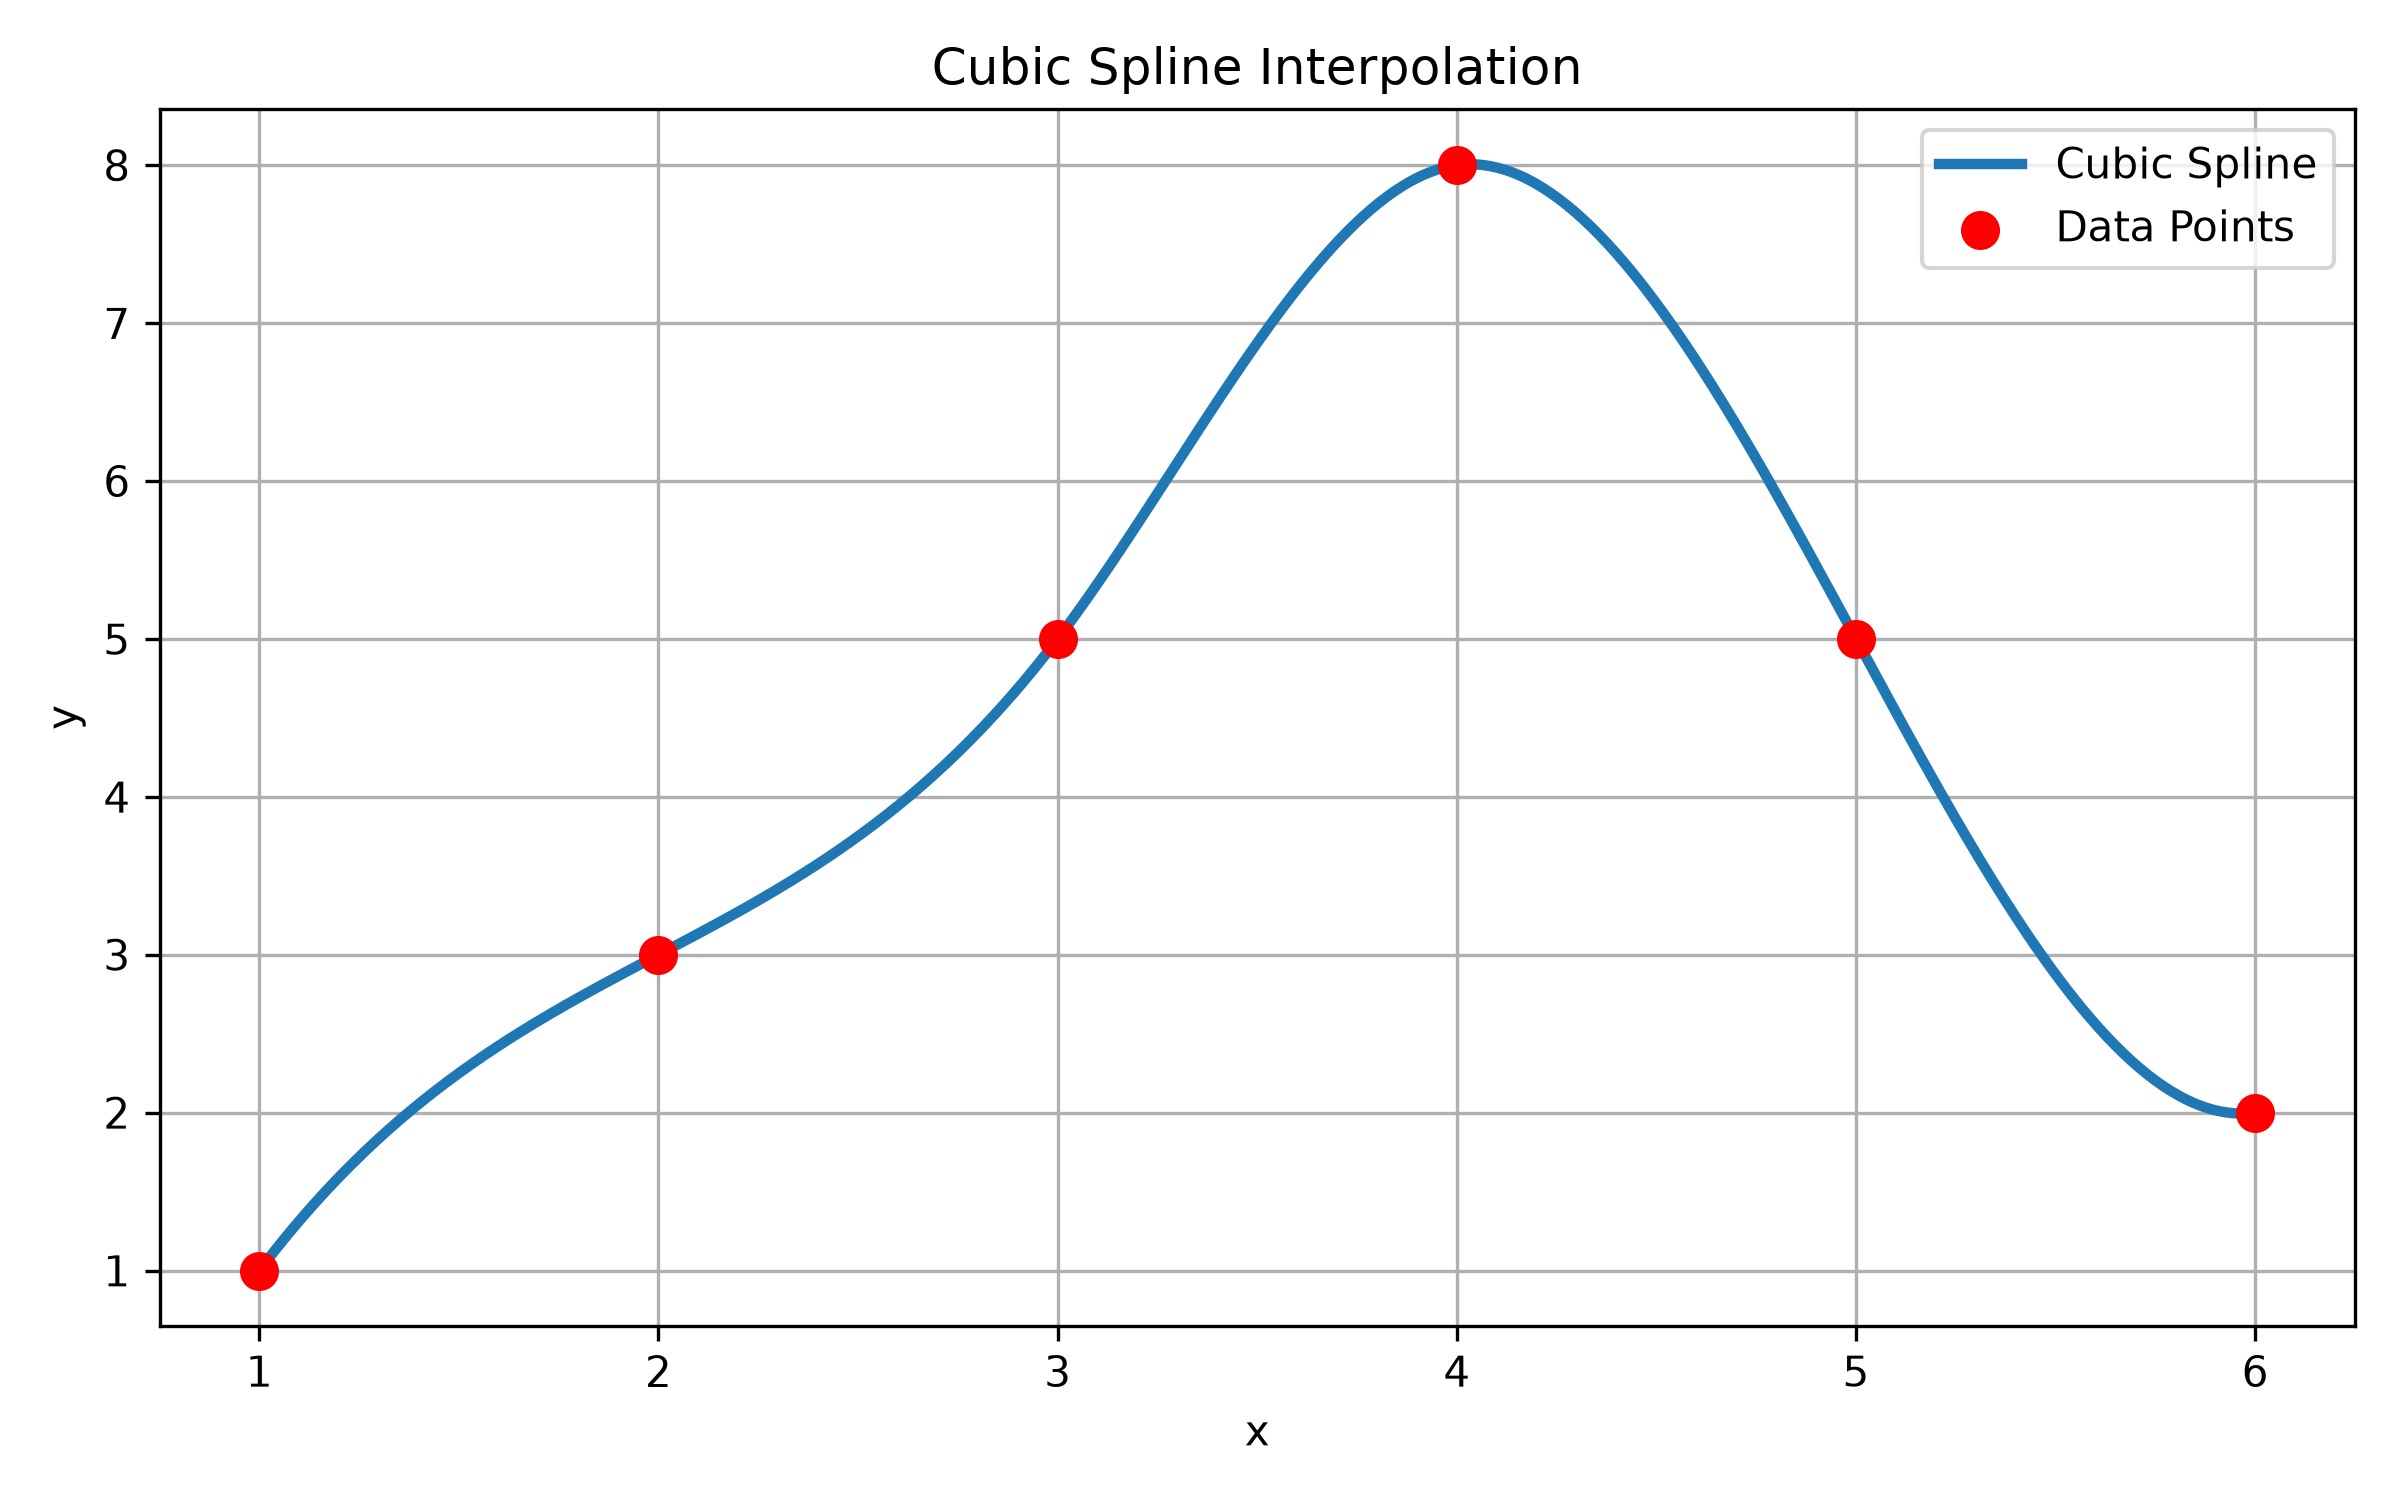
\includegraphics[width=0.82\textwidth]{figures/spline.png}
\caption{Cubic spline interpolation}
\label{fig:spline}
\end{figure}

در روش اسپلاین مکعبی، بازه بین هر دو نقطه توسط یک چندجمله‌ای درجه سه مدل‌سازی می‌شود. این چندجمله‌ای‌ها به گونه‌ای ساخته می‌شوند که علاوه بر عبور از تمامی نقاط، مشتق اول و دوم آن‌ها نیز در نقاط اتصال پیوسته باشد. در نتیجه، منحنی حاصل نسبت به لاگرانژ هموارتر بوده و رفتار پایدارتری دارد.

\subsection{مقایسه روش‌ها}

برای مقایسه بهتر دو روش، هر دو منحنی در یک نمودار رسم شده‌اند.

\begin{figure}[H]
\centering
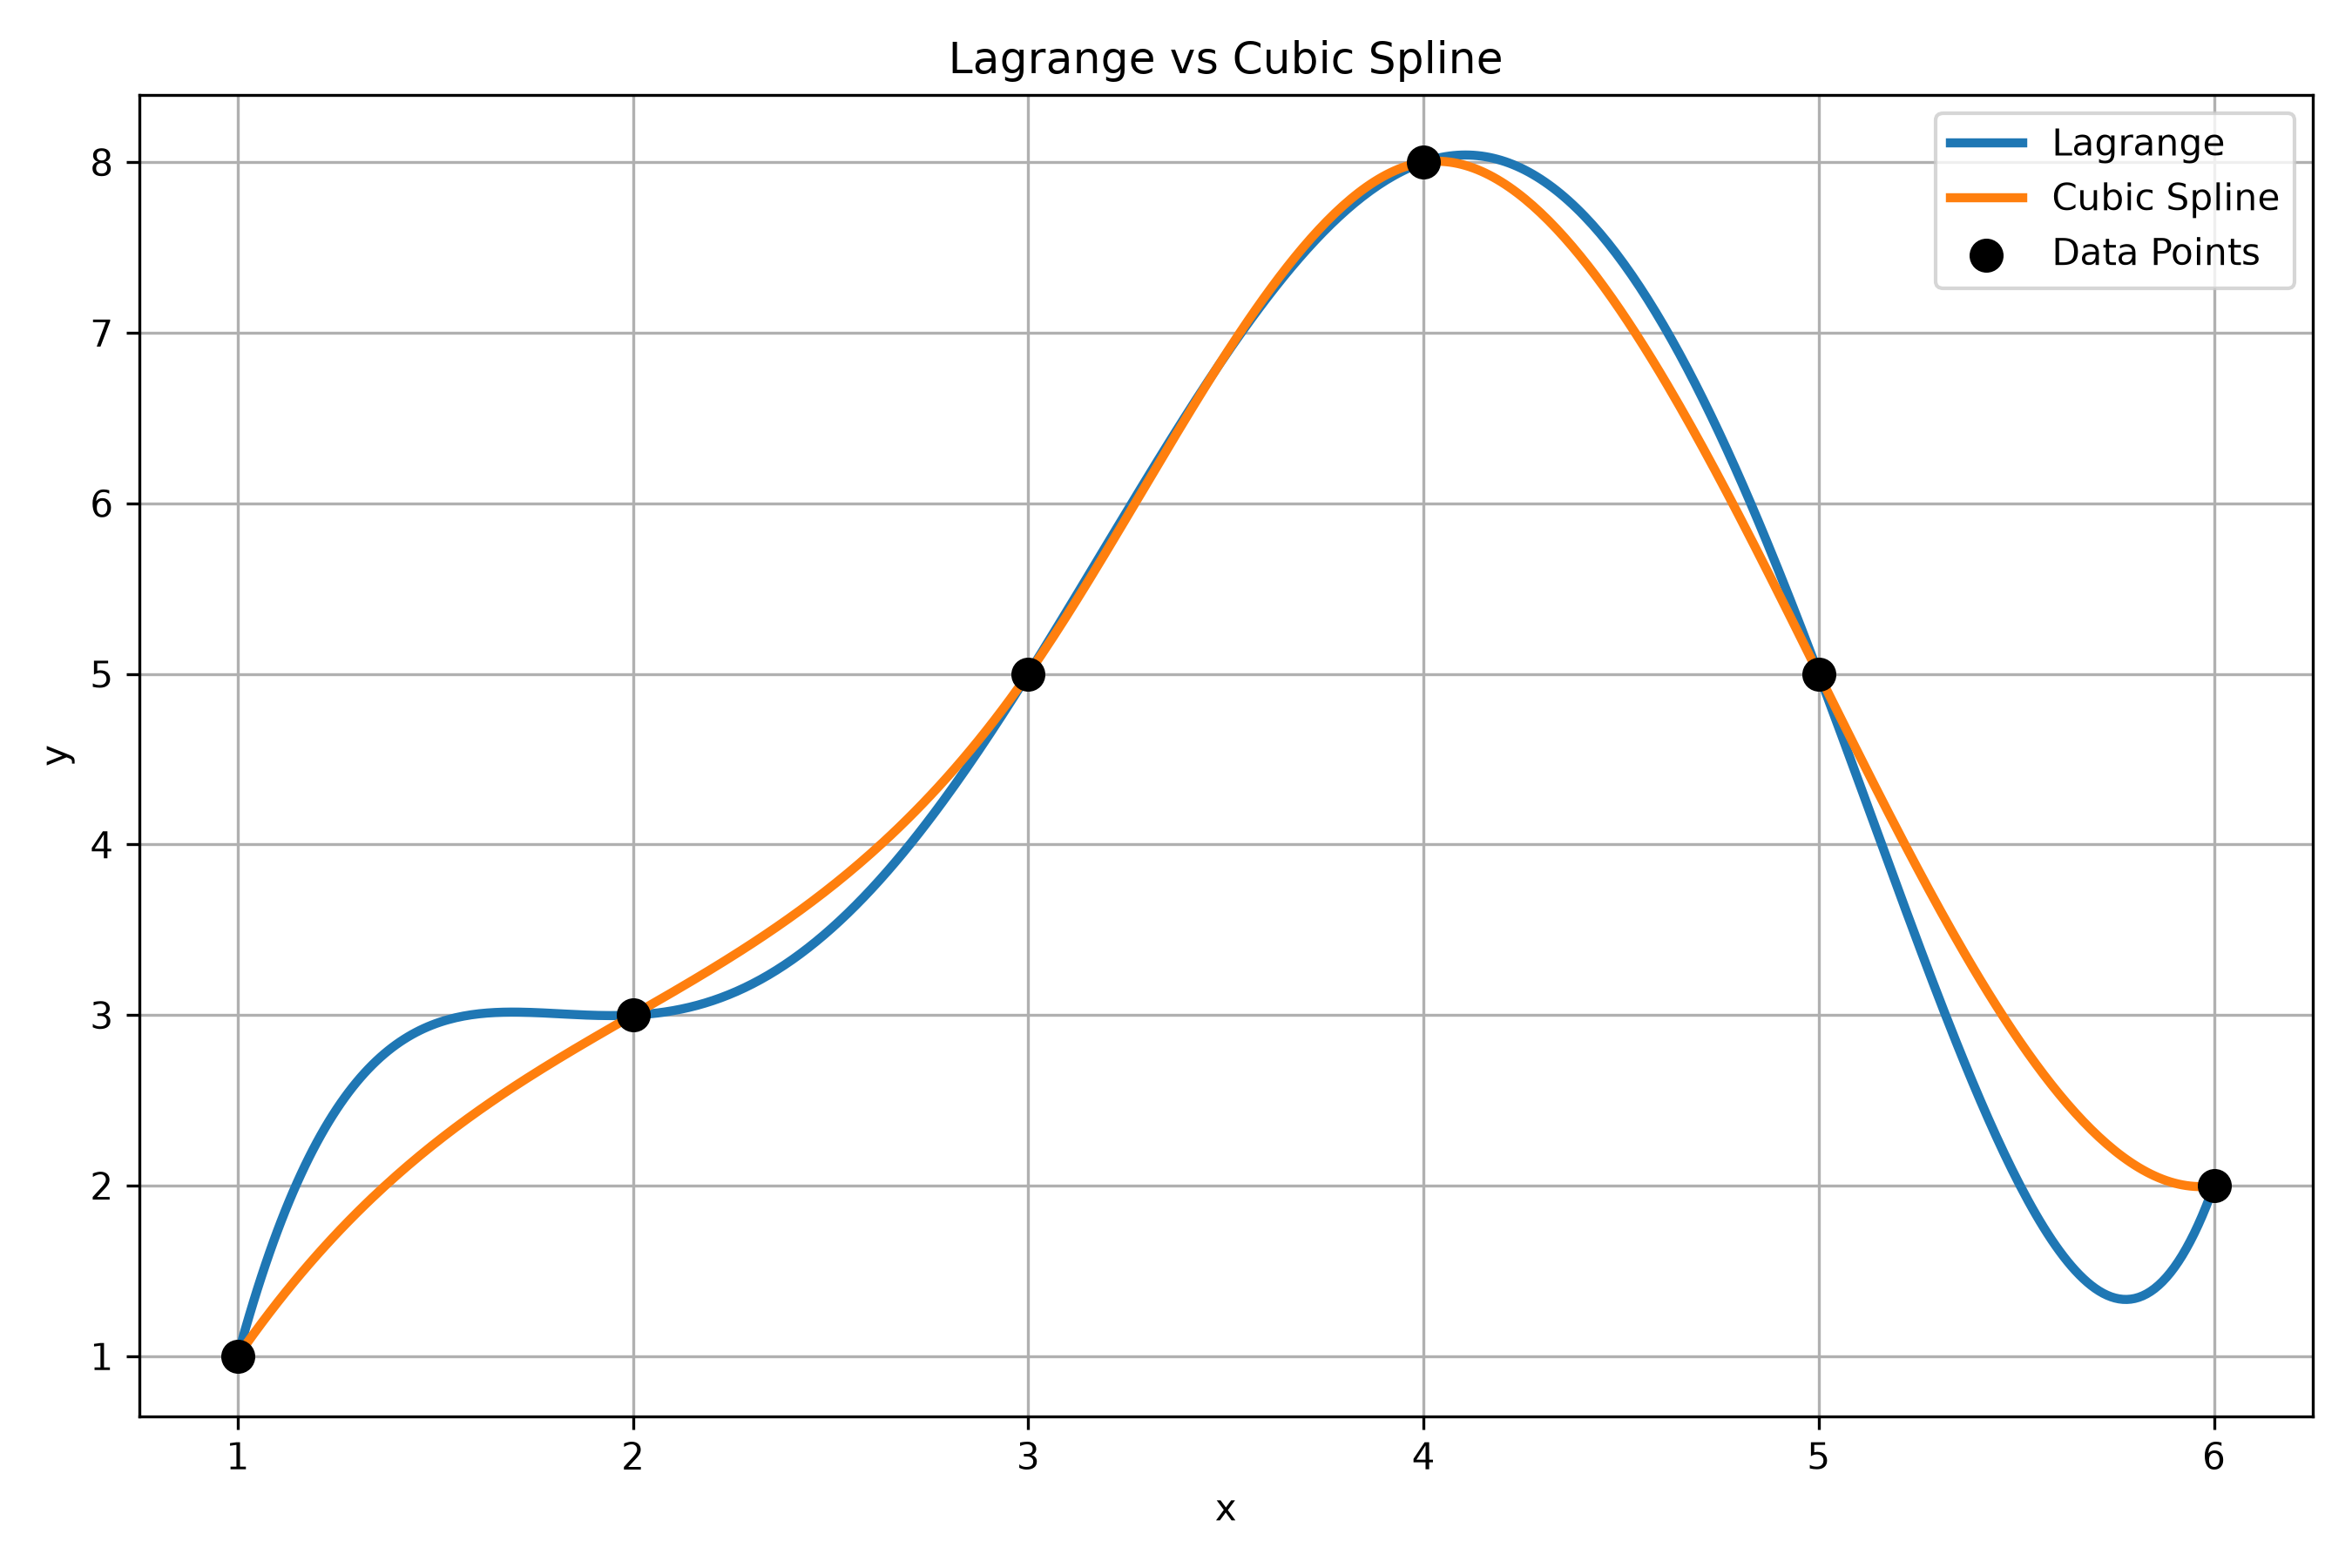
\includegraphics[width=0.9\textwidth]{figures/interpolation_comparison.png}
\caption{Comparison of Lagrange and Cubic Spline interpolation}
\label{fig:comparison}
\end{figure}

هر دو روش تمامی نقاط داده را به طور دقیق درونیابی می‌کنند، اما نحوه رفتار آن‌ها بین نقاط متفاوت است. در روش لاگرانژ تنها یک چندجمله‌ای سراسری وجود دارد، در حالی که در اسپلاین مکعبی هر بازه دارای یک چندجمله‌ای مستقل است. به همین دلیل، اسپلاین معمولاً نرمی بیشتر، پایداری عددی بهتر و حساسیت کمتری نسبت به افزایش تعداد نقاط دارد. به همین علت، برای بسیاری از کاربردهای مهندسی و علمی، استفاده از اسپلاین مکعبی نسبت به درونیابی لاگرانژ ترجیح داده می‌شود.


\section{سؤال دوم}

\subsection{صورت مسئله}

در این بخش، داده‌های مربوط به زمان اجرای سه الگوریتم مختلف برای اندازه‌های متفاوت داده ورودی از یک فایل اکسل خوانده شدند. هدف این بخش، رسم نمودارهای مختلف برای تحلیل داده‌ها، بررسی رفتار الگوریتم‌ها و محاسبه میانگین زمان اجرای الگوریتم دوم است. تمامی داده‌ها به صورت مستقیم از فایل اکسل خوانده شده‌اند و هیچ مقداری به صورت دستی در برنامه وارد نشده است.

\subsection{خواندن فایل اکسل}

ابتدا فایل اکسل با استفاده از کتابخانه \lr{Pandas} خوانده شد. سپس سطرهای خالی حذف شده و داده‌ها برای تحلیل آماده شدند. با توجه به نحوه پیاده‌سازی برنامه، تعداد سطرها و ستون‌های فایل به صورت خودکار تشخیص داده می‌شود؛ بنابراین در صورت اضافه شدن داده‌های جدید، بدون ایجاد تغییر در کد، تمامی نمودارها مجدداً با داده‌های جدید رسم خواهند شد.

\subsection{نمودار میله‌ای}

\begin{figure}[H]
\centering
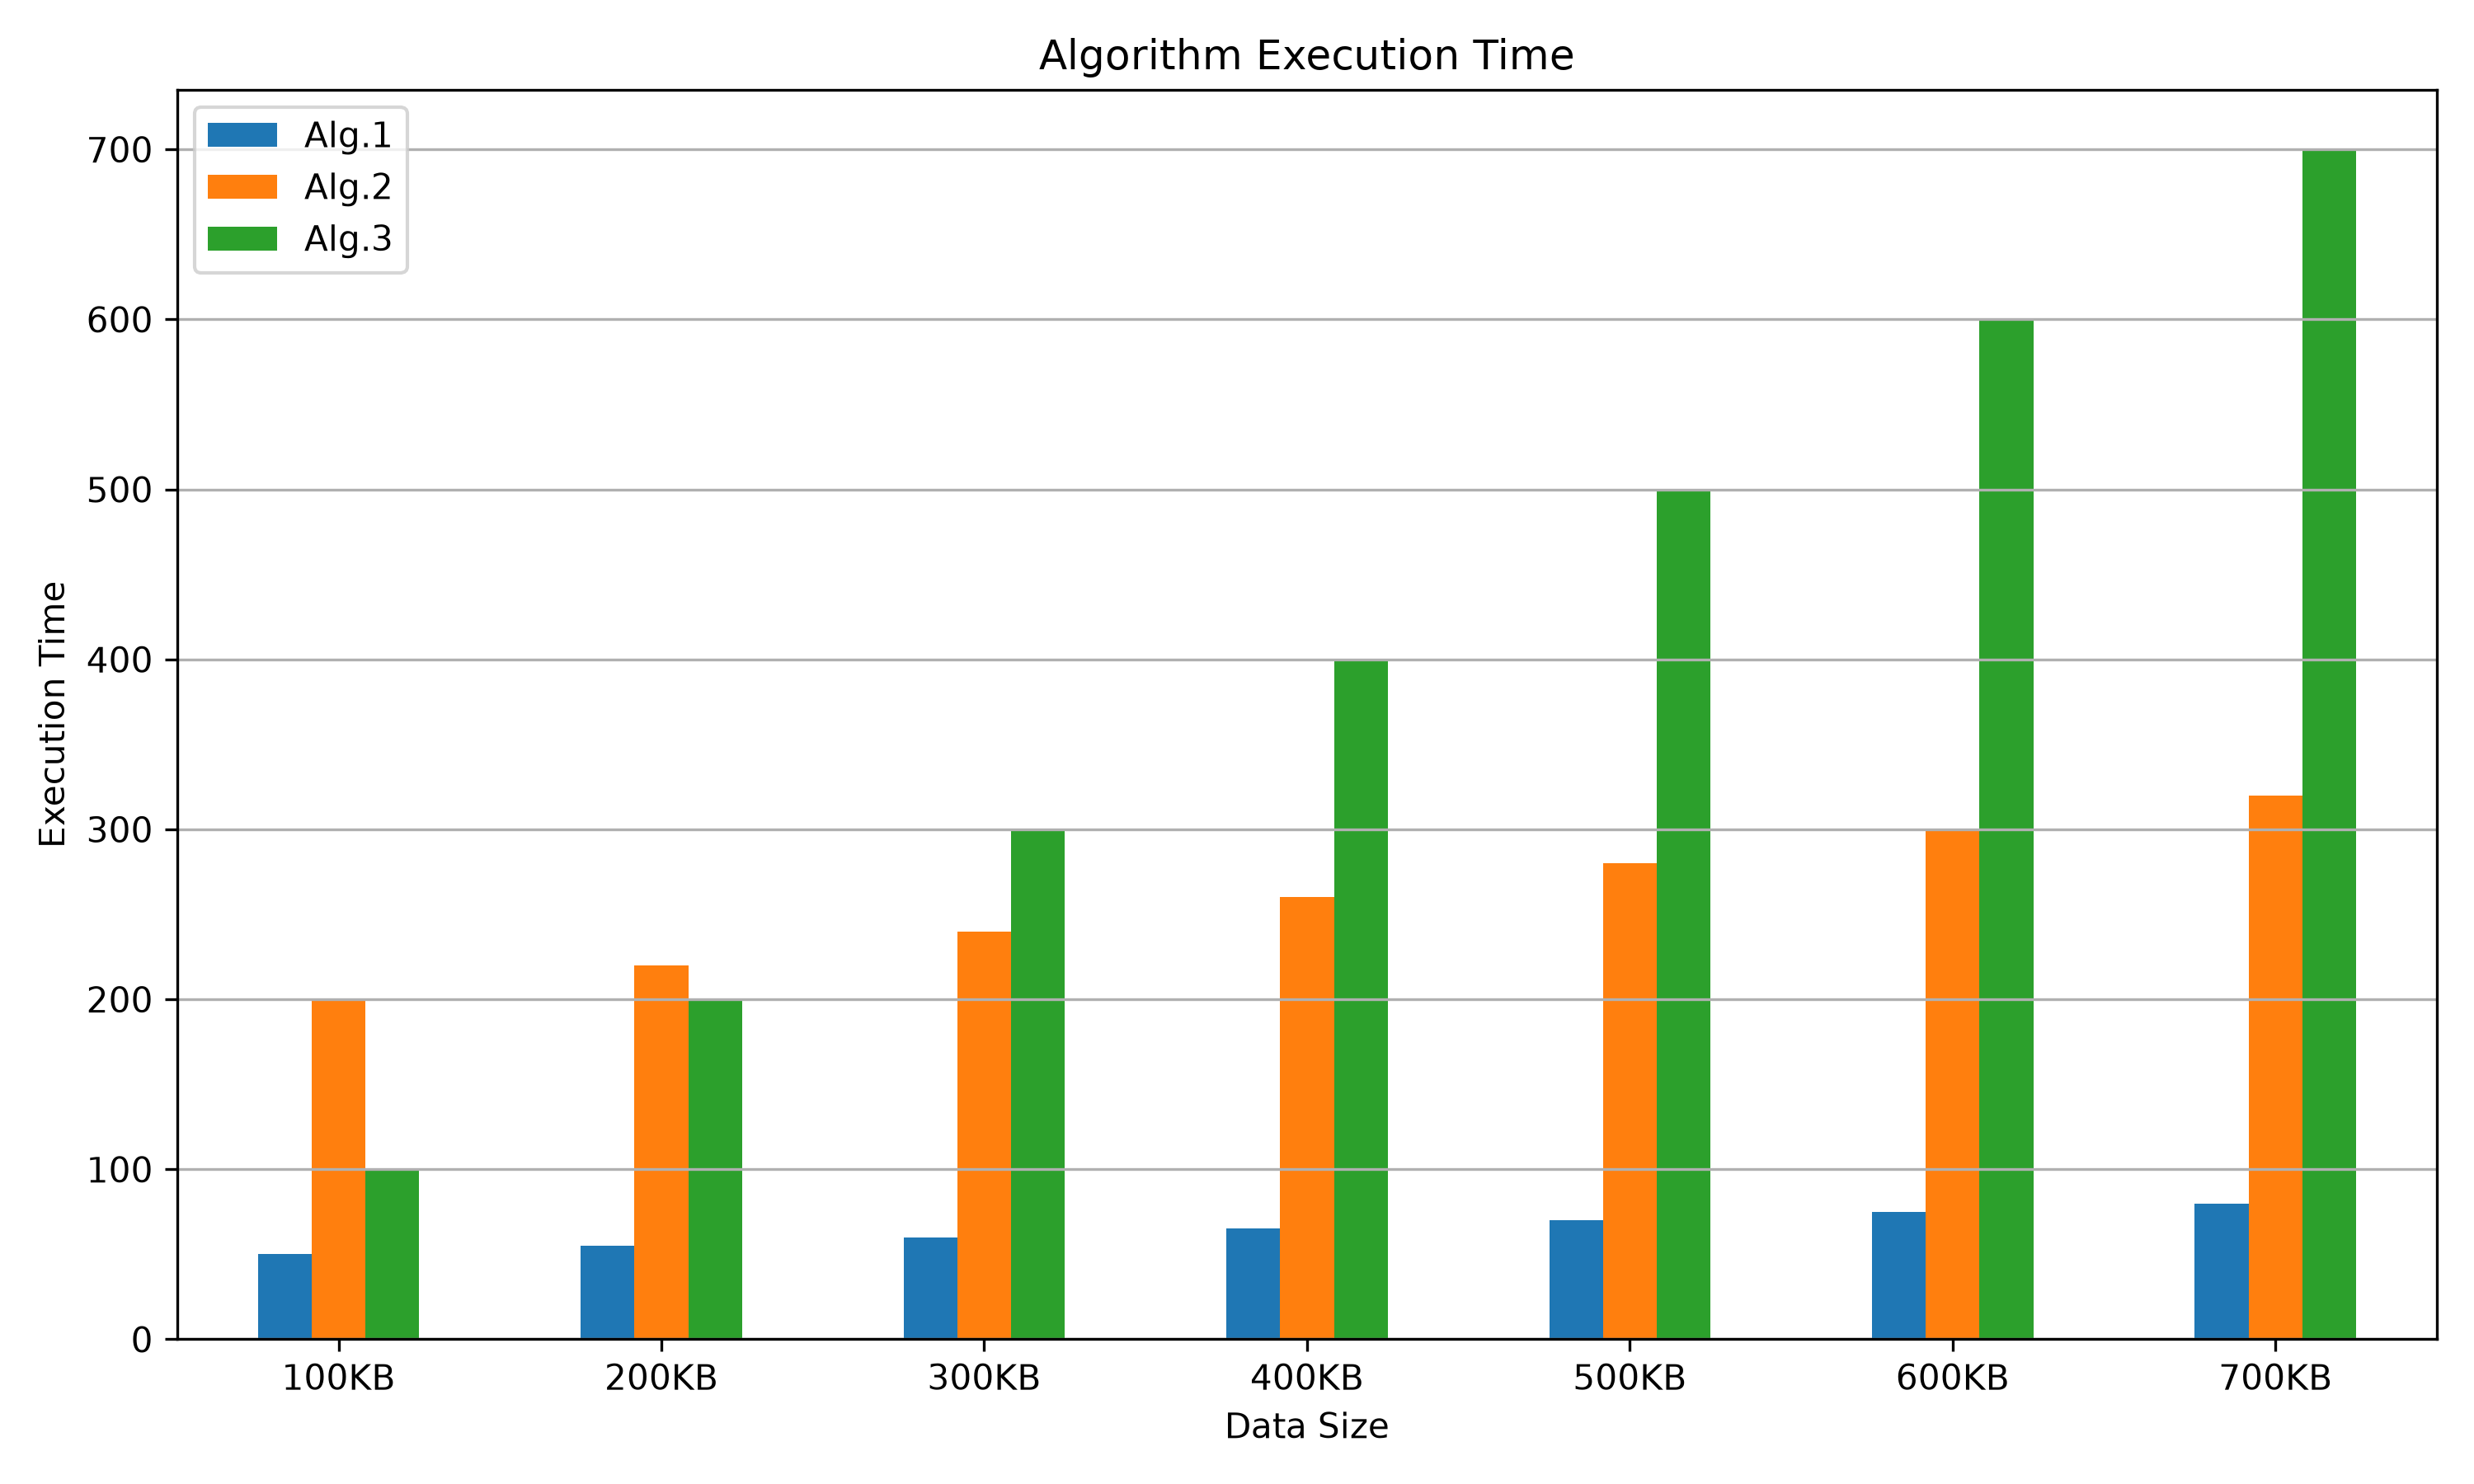
\includegraphics[width=.9\textwidth]{figures/bar_chart.png}
\caption{Bar chart of algorithm execution times}
\label{fig:bar}
\end{figure}

نمودار میله‌ای امکان مقایسه مستقیم زمان اجرای سه الگوریتم را برای هر اندازه داده فراهم می‌کند. با افزایش اندازه داده‌ها، زمان اجرای هر سه الگوریتم روندی افزایشی دارد، اما نرخ افزایش آن‌ها یکسان نیست. الگوریتم اول کمترین زمان اجرا را در تمامی اندازه‌های داده دارد، در حالی که الگوریتم سوم بیشترین زمان اجرا را نشان می‌دهد.

\subsection{نمودار خطی}

\begin{figure}[H]
\centering
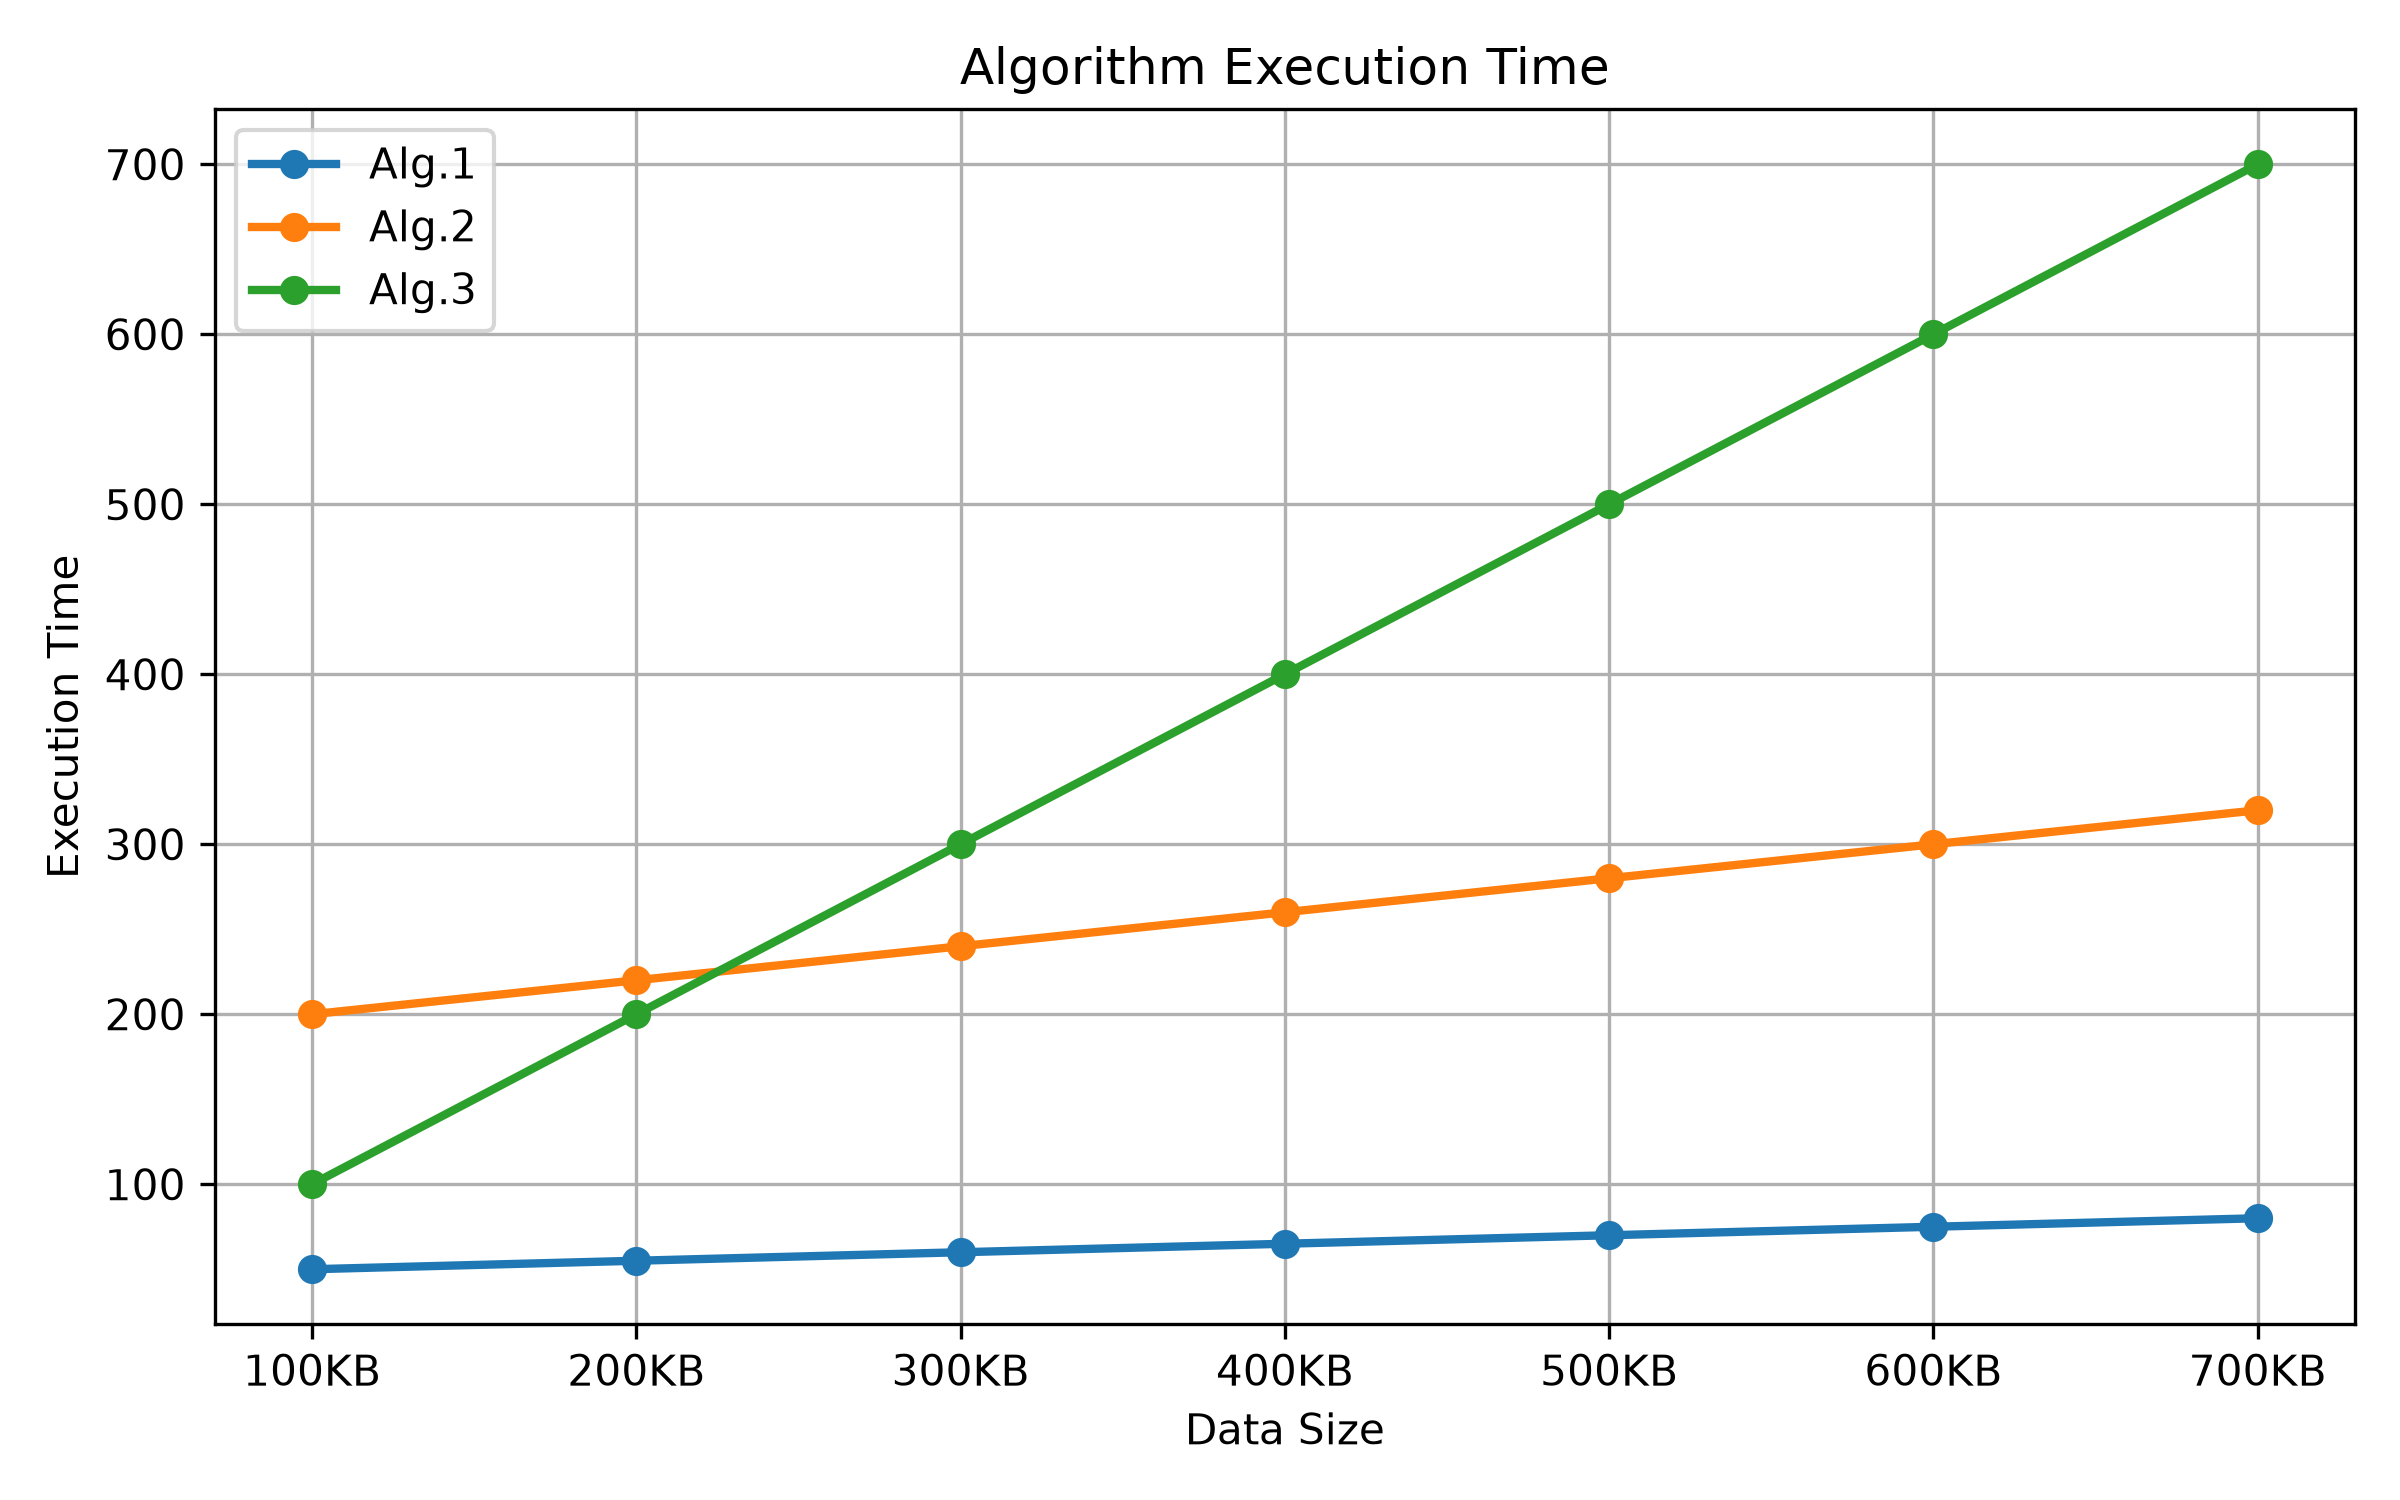
\includegraphics[width=.9\textwidth]{figures/line_chart.png}
\caption{Line chart of algorithm execution times}
\label{fig:line}
\end{figure}

نمودار خطی روند تغییرات زمان اجرای هر الگوریتم را با افزایش اندازه داده نمایش می‌دهد. مشاهده می‌شود که هر سه الگوریتم دارای روندی صعودی هستند، اما شیب افزایش زمان اجرا برای الگوریتم سوم بیشتر از دو الگوریتم دیگر است. این موضوع نشان می‌دهد که با افزایش حجم داده، اختلاف عملکرد الگوریتم‌ها نیز بیشتر می‌شود.

\subsection{نمودار جعبه‌ای}

\begin{figure}[H]
\centering
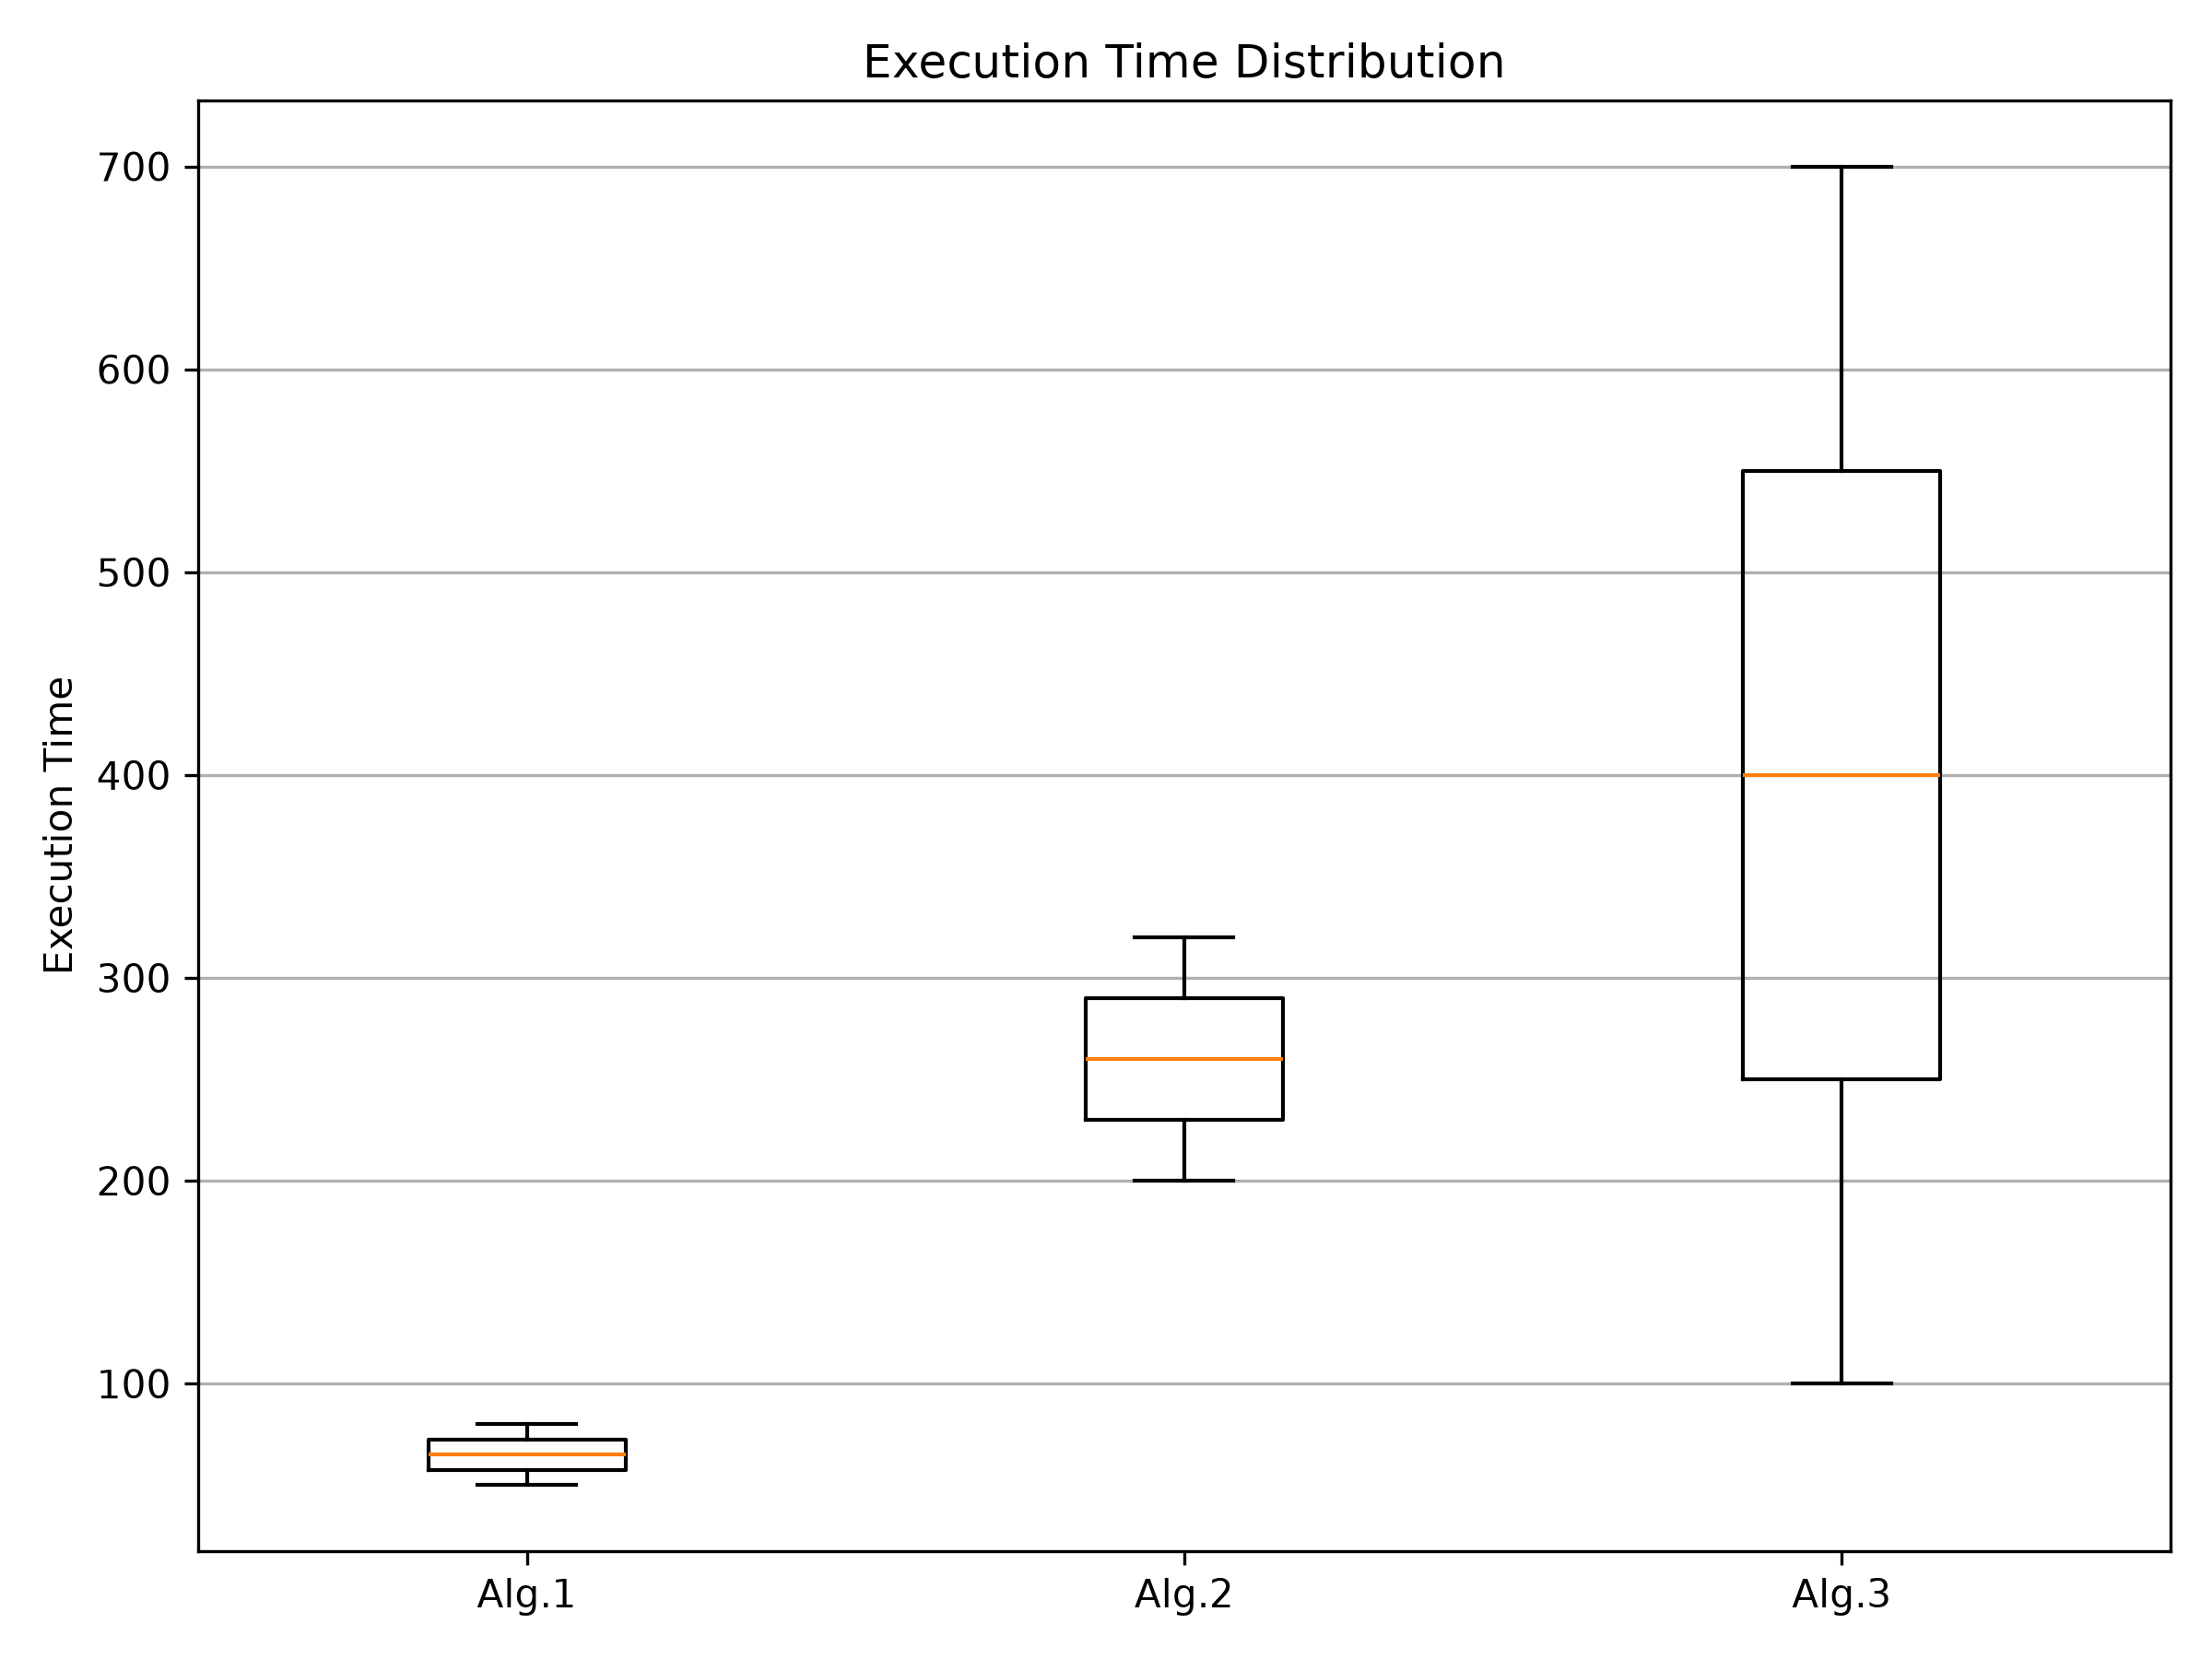
\includegraphics[width=.8\textwidth]{figures/box_plot.png}
\caption{Box plot of algorithm execution times}
\label{fig:box}
\end{figure}

نمودار جعبه‌ای توزیع زمان اجرای هر الگوریتم را نمایش می‌دهد. محل قرارگیری میانه، دامنه بین چارکی و گستردگی داده‌ها نشان می‌دهد که الگوریتم سوم علاوه بر داشتن بیشترین زمان اجرا، بیشترین پراکندگی را نیز دارد. در مقابل، الگوریتم اول دارای کمترین پراکندگی و پایدارترین عملکرد در میان سه الگوریتم است.

\subsection{میانگین زمان اجرای الگوریتم دوم}

در این قسمت، مقادیر مربوط به ستون الگوریتم دوم برای اندازه‌های داده بین 100 تا 600 کیلوبایت از فایل اکسل استخراج شده و میانگین آن‌ها محاسبه گردید.

میانگین زمان اجرای الگوریتم دوم برابر با \lr{190} واحد زمانی به دست آمد. این مقدار بیانگر عملکرد متوسط الگوریتم دوم بر روی مجموعه داده‌های موجود در فایل اکسل است.

\subsection{جمع‌بندی}

نتایج این بخش نشان داد که استفاده از کتابخانه‌های تحلیلی پایتون مانند \lr{Pandas} و \lr{Matplotlib} امکان خواندن خودکار داده‌ها، رسم نمودارهای متنوع و انجام تحلیل‌های آماری را به سادگی فراهم می‌کند. همچنین پیاده‌سازی انجام‌شده به گونه‌ای است که با اضافه شدن داده‌های جدید به فایل اکسل، تمامی نمودارها و محاسبات بدون نیاز به تغییر در کد به‌روزرسانی خواهند شد.

\section{سؤال سوم}

\subsection{صورت مسئله}

در این بخش، مقدار انتگرال معین تابع

\[
f(x)=e^{x^2}
\]

بر روی بازه

\[
[0,1]
\]

با استفاده از سه روش مختلف انتگرال‌گیری عددی محاسبه شده است. روش‌های مورد استفاده شامل روش ذوزنقه‌ای، روش سیمپسون و انتگرال‌گیری گاوسی هستند. در انتها نیز نتایج حاصل از این روش‌ها با یکدیگر مقایسه شده‌اند.

\subsection{رسم تابع}

ابتدا تابع مورد نظر بر روی بازه $[0,1]$ رسم شد تا رفتار آن پیش از انجام انتگرال‌گیری بررسی شود.

\begin{figure}[H]
\centering
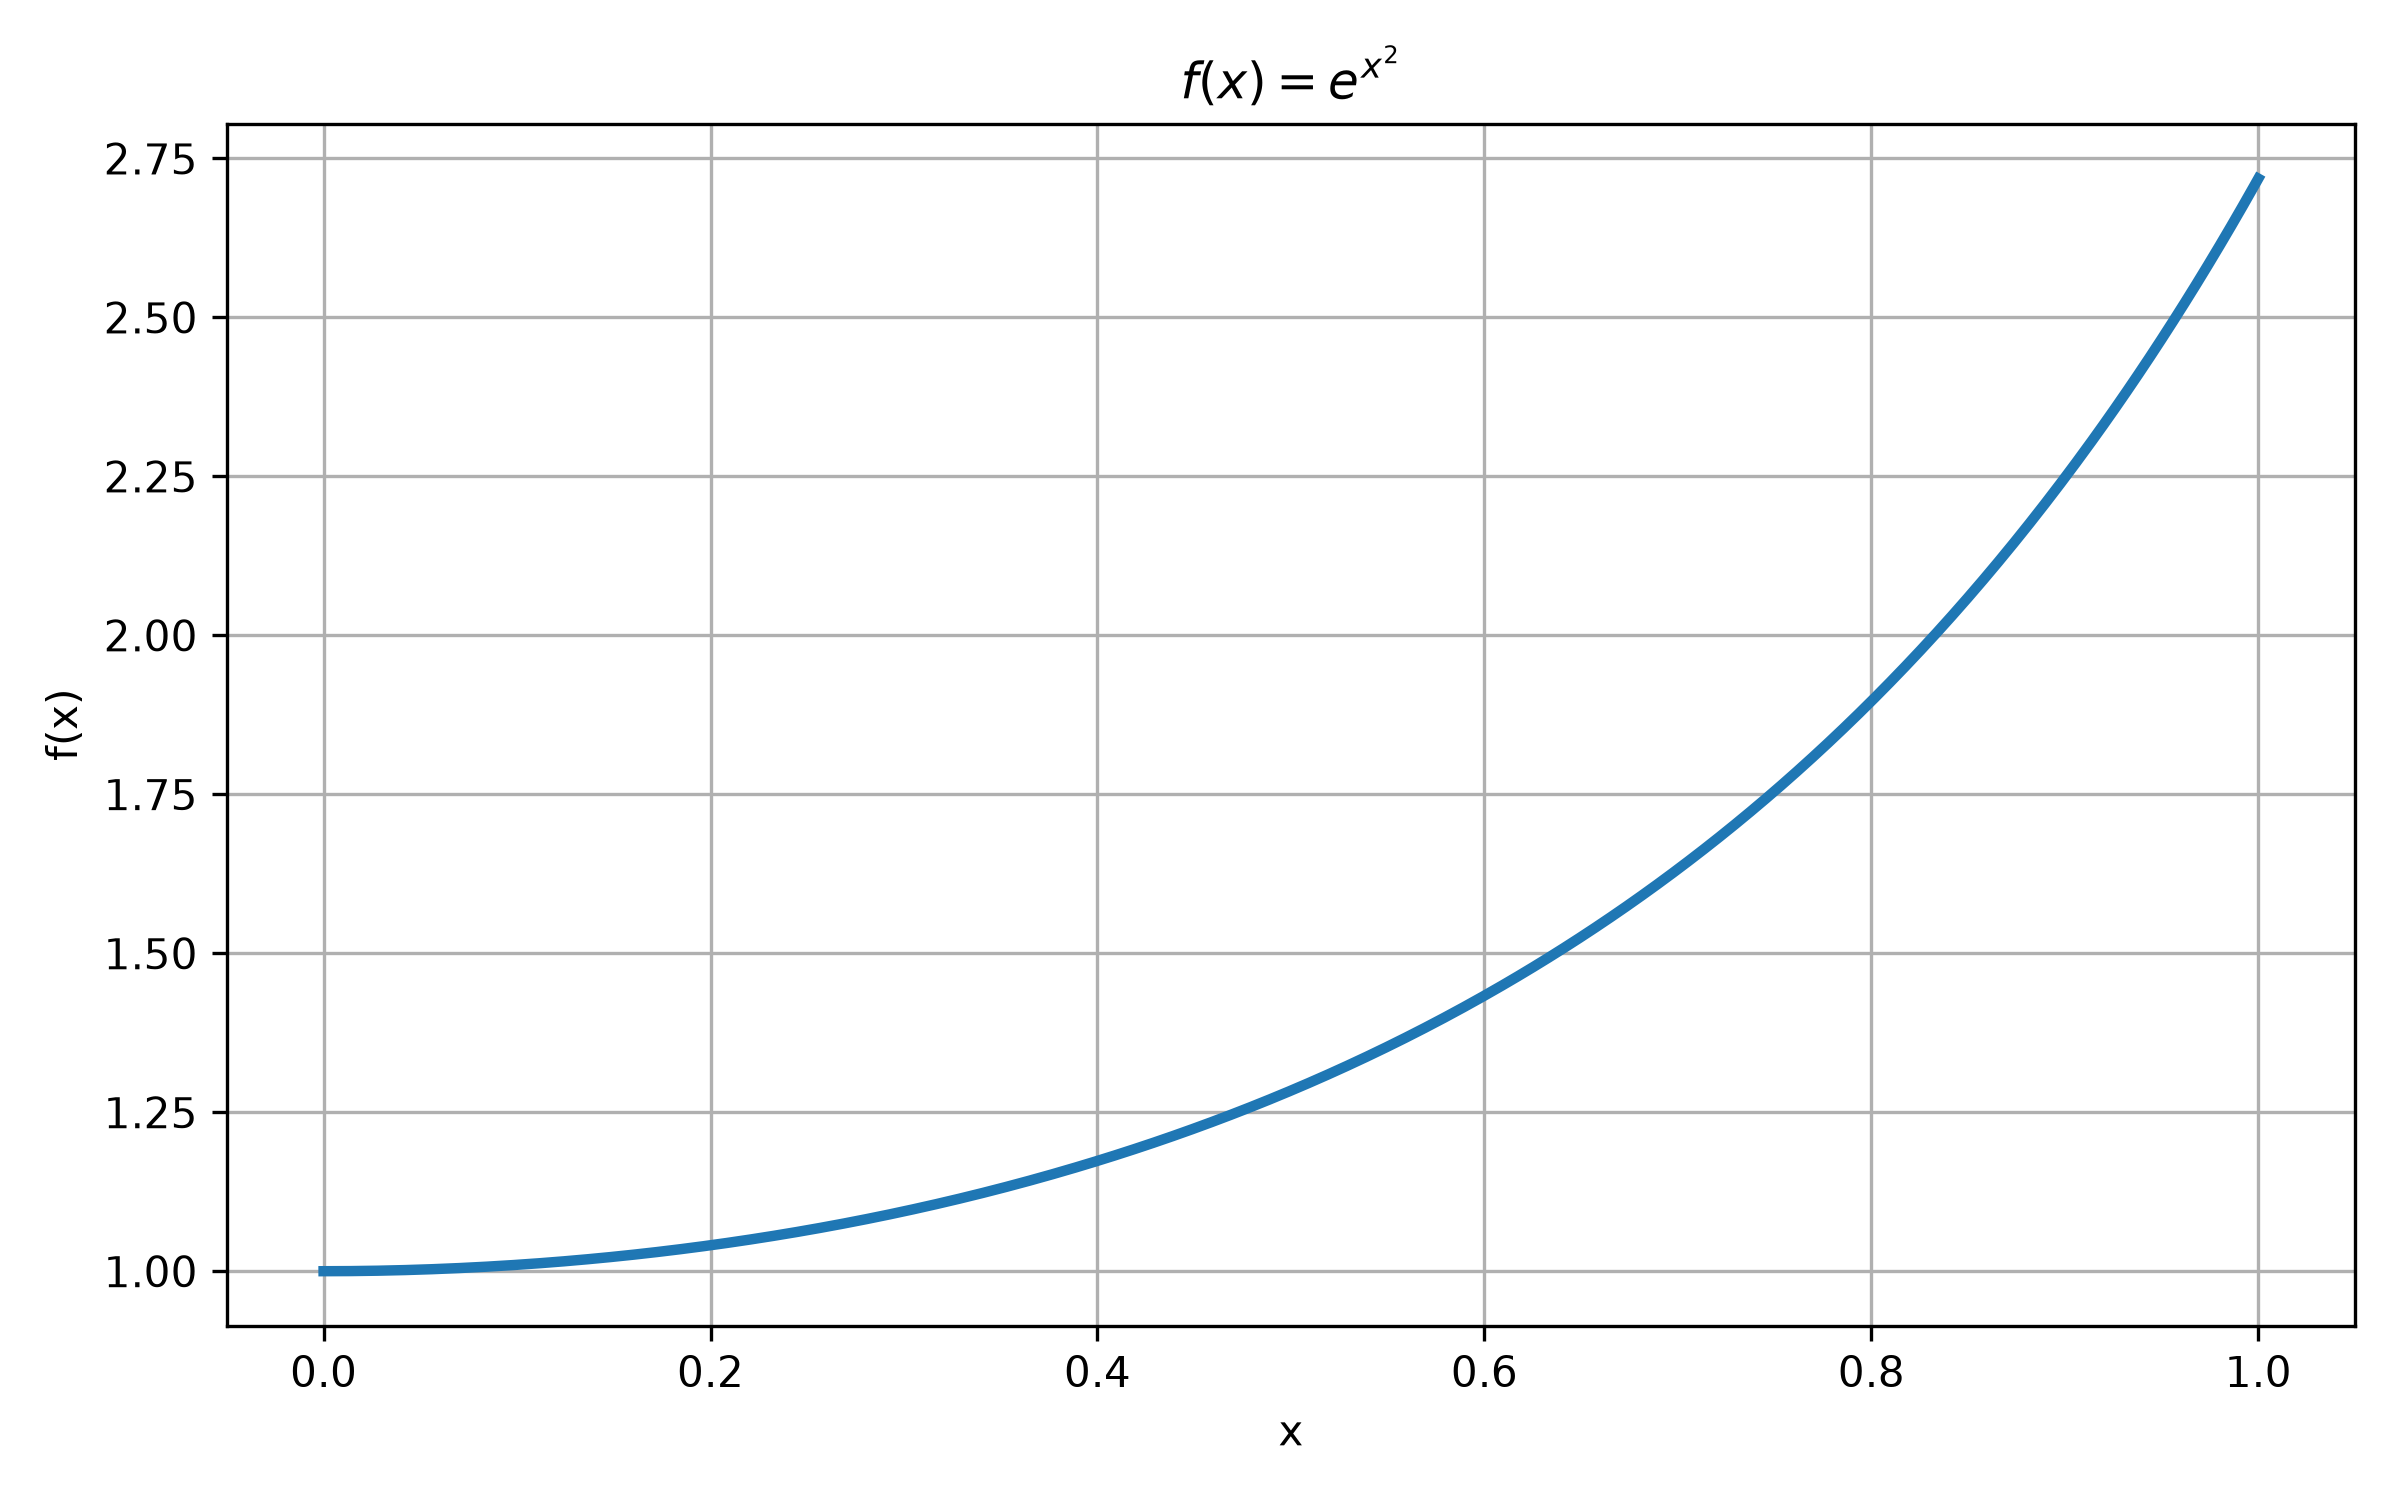
\includegraphics[width=.78\textwidth]{figures/function_plot.png}
\caption{Plot of $f(x)=e^{x^2}$ over the interval $[0,1]$}
\label{fig:function}
\end{figure}

مطابق شکل، تابع در کل بازه مقداری مثبت داشته و روندی صعودی دارد. همچنین آهنگ افزایش تابع با بزرگ‌تر شدن مقدار $x$ بیشتر می‌شود که ناشی از وجود تابع نمایی است.

\subsection{روش ذوزنقه‌ای}

در این روش، بازه انتگرال به تعدادی زیر‌بازه مساوی تقسیم شده و مساحت زیر نمودار با استفاده از مجموع مساحت ذوزنقه‌های تشکیل‌شده تقریب زده می‌شود.

مقدار تقریبی انتگرال با استفاده از روش ذوزنقه‌ای برابر است با

\[
I_T=\text{\lr{1.4626970498}}
\]

\subsection{روش سیمپسون}

در روش سیمپسون، در هر زیر‌بازه از یک چندجمله‌ای درجه دو برای تقریب تابع استفاده می‌شود. به همین دلیل این روش معمولاً نسبت به روش ذوزنقه‌ای دقت بیشتری دارد.

مقدار تقریبی انتگرال با استفاده از روش سیمپسون برابر است با

\[
I_S=\text{\lr{1.4626517489}}
\]

\subsection{انتگرال‌گیری گاوسی}

در این قسمت، انتگرال با استفاده از روش گاوسی محاسبه شد. این روش با انتخاب مناسب نقاط نمونه‌برداری و ضرایب متناظر، دقت بسیار بالایی را با تعداد کمی نقطه فراهم می‌کند.

مقدار تقریبی انتگرال با استفاده از انتگرال‌گیری گاوسی برابر است با

\[
I_G=\text{\lr{1.4626516680}}
\]

\subsection{مقایسه نتایج}

برای مقایسه بهتر روش‌های مختلف، نتایج محاسبه‌شده در قالب یک جدول خلاصه شده‌اند.

\begin{table}[H]
\centering
\caption{Comparison of numerical integration methods}
\begin{tabular}{|c|c|}
\hline
\textbf{Method} & \textbf{Integral Value} \\
\hline
Trapezoidal Rule & \lr{1.462697} \\
\hline
Simpson's Rule & \lr{1.462652} \\
\hline
Gaussian Quadrature & \lr{1.462652} \\
\hline
\end{tabular}
\end{table}

نتایج به‌دست‌آمده نشان می‌دهند که هر سه روش مقدار تقریبی بسیار نزدیکی برای انتگرال ارائه می‌کنند. با این حال، روش گاوسی بیشترین دقت را دارد، زیرا با استفاده از نقاط و وزن‌های بهینه مقدار انتگرال را تقریب می‌زند. روش سیمپسون نیز دقت بسیار مناسبی داشته و نتیجه آن تقریباً با مقدار روش گاوسی منطبق است. در مقابل، روش ذوزنقه‌ای به دلیل استفاده از تقریب خطی در هر زیر‌بازه، دارای خطای بیشتری نسبت به دو روش دیگر است. بنابراین، در این مسئله استفاده از روش گاوسی و سپس روش سیمپسون بهترین نتایج را ارائه می‌دهد.

\section{جمع‌بندی}

در این پروژه، سه مبحث مهم از درس نرم‌افزار ریاضی با استفاده از زبان برنامه‌نویسی Python پیاده‌سازی و بررسی شدند.

در بخش اول، دو روش درونیابی لاگرانژ و اسپلاین مکعبی برای تقریب مجموعه‌ای از داده‌های گسسته مورد استفاده قرار گرفتند. نتایج نشان داد که هر دو روش قادر به عبور دقیق از تمامی نقاط داده هستند، اما اسپلاین مکعبی به دلیل ساختار قطعه‌ای خود، منحنی هموارتر و پایدارتری تولید می‌کند.

در بخش دوم، داده‌های موجود در یک فایل اکسل به صورت خودکار خوانده شده و نمودارهای میله‌ای، خطی و جعبه‌ای برای تحلیل زمان اجرای سه الگوریتم مختلف رسم شدند. همچنین میانگین زمان اجرای الگوریتم دوم محاسبه گردید. پیاده‌سازی انجام‌شده به گونه‌ای است که با اضافه شدن داده‌های جدید به فایل اکسل، تمامی نمودارها بدون نیاز به تغییر در کد به‌روزرسانی می‌شوند.

در بخش سوم، مقدار انتگرال تابع $e^{x^2}$ در بازه $[0,1]$ با استفاده از روش‌های ذوزنقه‌ای، سیمپسون و انتگرال‌گیری گاوسی محاسبه شد. مقایسه نتایج نشان داد که روش گاوسی بیشترین دقت را ارائه می‌دهد و روش سیمپسون نیز عملکرد بسیار مناسبی دارد.

به طور کلی، این پروژه نشان داد که کتابخانه‌های علمی Python ابزارهای قدرتمندی برای حل مسائل مربوط به درونیابی، تحلیل داده و محاسبات عددی فراهم می‌کنند و می‌توانند در پیاده‌سازی روش‌های مختلف نرم‌افزار ریاضی با دقت و کارایی بالا مورد استفاده قرار گیرند.

\section{GitHub}

مطابق صورت پروژه، تمامی کدهای مربوط به پروژه‌های درس در یک مخزن عمومی GitHub قرار گرفته‌اند.

لینک مخزن:

\begin{center}
\url{https://github.com/ParsaNasirii/MS_Project3_40212047_Nasiri}
\end{center}

\end{document}